\documentclass[final,12pt]{colt2018}

\title{Online learning over a finite action set with limited switching}
% % Authors with different addresses:
\coltauthor{\Name{Jason Altschuler} \Email{jasonalt@mit.edu}\\
\addr Massachusetts Institute of Technology
\AND
\Name{Kunal Talwar} \Email{kunal@google.com}\\
\addr Google Brain
}

% % TODO: mention some of these results were presented in JA's undergrad thesis at Princeton.




%replacement usepackages for removing the colt styl.
%\usepackage{amsmath,amssymb,graphicx,url}
%\usepackage{graphicx}
%\usepackage{subfigure}
%\usepackage[boxed]{algorithm2e}

%\usepackage{amsthm}
%\newtheorem{theorem}{Theorem}
%\newtheorem{corollary}[theorem]{Corollary}
%\newtheorem{lemma}[theorem]{Lemma}
%\newtheorem{proposition}[theorem]{Proposition}
%\newtheorem{definition}{Definition}
%\newtheorem{remark}[theorem]{Remark}

%\usepackage{times}
\usepackage{enumitem}
\usepackage{framed}
\usepackage{multirow}
\usepackage{bm}
\usepackage{float}
\usepackage{color}

%\usepackage[round,comma]{natbib}
%\bibliographystyle{plainnat}


% added for arxiv version
%\usepackage[margin=1.3in]{geometry} 

\usepackage{hyperref}       % hyperlinks
\usepackage{url}            % simple URL typesetting
\usepackage{booktabs}       % professional-quality tables
\usepackage{nicefrac}       % compact symbols for 1/2, etc.
\usepackage{microtype}      % microtypography
\usepackage{framed}

% ----------------------------------------------
% ---< Uncomment to turn back into COLT sty >---
% ----------------------------------------------
\PassOptionsToPackage{boxed}{algorithm2e}%
%\documentclass[anon,12pt]{colt2018} % Anonymized submission
%\usepackage{times}
% \coltauthor{
%         \Name{Jason Altschuler}
%         Massachusetts Institute of Technology\\
%         77 Massachusetts Avenue\\
%         Cambridge, MA 02139-4307, USA
%         \AND
%         \Name{Victor-Emmanuel Brunel}
%         Massachusetts Institute of Technology\\
%         77 Massachusetts Avenue\\
%         Cambridge, MA 02139-4307, USA
%         \Name{Alan Malek} \Email{amalek@mit.edu}\\
%         \addr
%         Massachusetts Institute of Technology\\
%         77 Massachusetts Avenue\\
%         Cambridge, MA 02139-4307, USA
%       }

% ----------------------------------------------
% --<\ Uncomment to turn back into COLT sty >---
% ----------------------------------------------



\DeclareMathOperator{\Real}{\mathbb{R}}
\DeclareMathOperator*{\argmin}{arg\,min}
\DeclareMathOperator*{\argmax}{arg\,max}
\DeclareMathOperator{\E}{\mathbb{E}}
\DeclareMathOperator{\F}{\mathcal{F}}
\DeclareMathOperator{\Prob}{\mathbb{P}}
\DeclareMathOperator{\half}{\tfrac{1}{2}}

\DeclareMathOperator{\Ber}{\text{Ber}}
\DeclareMathOperator{\Bin}{\text{Bin}}
\DeclareMathOperator{\Exp}{\text{Exp}}

\DeclareMathOperator{\eps}{\varepsilon}
\DeclareMathOperator{\logdel}{\log\tfrac{1}{\delta}}
\DeclareMathOperator{\logtdel}{\log\tfrac{2}{\delta}}
\DeclareMathOperator{\halfdel}{\tfrac{\delta}{2}}

\DeclareMathOperator{\asleq}{\overset{\text{a.s.}}{\leq}}
\DeclareMathOperator{\asgeq}{\overset{\text{a.s.}}{\geq}}

\DeclareMathOperator{\Regret}{\text{Regret}}
\DeclareMathOperator{\Regretunclipped}{\text{Regret}^{\text{unclipped}}}
\DeclareMathOperator{\elltunclipped}{\ell_t^{\text{unclipped}}}
\DeclareMathOperator{\hatl}{\hat{\ell}}
\DeclareMathOperator{\numswitches}{\text{\# switches}}
\DeclareMathOperator{\Switches}{\text{Switches}}
\DeclareMathOperator{\Ltarg}{L_\text{target}}


\DeclareMathOperator{\pfe}{\text{PFE}}
\DeclareMathOperator{\mab}{\text{MAB}}

\DeclareMathOperator{\sd}{\textsc{SD}}

\DeclareMathOperator{\btl}{\textsc{BTL}}
\DeclareMathOperator{\ftl}{\textsc{FTL}}

\DeclareMathOperator{\fpl}{\textsc{FPL}}
\DeclareMathOperator{\fll}{\textsc{FLL}}
\DeclareMathOperator{\bfll}{\textsc{BFLL}}

\DeclareMathOperator{\mfpl}{\textsc{FPL}^*}
\DeclareMathOperator{\mfpleps}{\textsc{FPL}_{\eps}^*}
\DeclareMathOperator{\bmfpl}{\textsc{BFPL}_{\delta}^*}

\DeclareMathOperator{\pr}{\textsc{PRW}}
\DeclareMathOperator{\bpr}{\textsc{BPRW}}

\DeclareMathOperator{\cpr}{\textsc{CombPRW}}
\DeclareMathOperator{\bcpr}{\textsc{BCombPRW}}

\DeclareMathOperator{\calA}{\mathcal{A}}
\DeclareMathOperator{\calB}{\mathcal{B}}
\DeclareMathOperator{\calF}{\mathcal{F}}

\DeclareMathOperator{\PEV}{\textsc{PEV}}
\DeclareMathOperator{\SEV}{\textsc{SEV}}

\newcommand{\plusminus}{\raisebox{.2ex}{$\scriptstyle\pm$}}

\newcommand{\freefootnote}[1]{{%
  \let\thempfn\relax% Remove footnote number printing mechanism
  \footnotetext[0]{\emph{#1}}% Print footnote text
}}

%\author{
%        Jason Altschuler\\
%        Massachusetts Institute of Technology\\
%        \texttt{jasonalt@mit.edu}
%        \and
%        Kunal Talwar\\
%        Google Brain\\
%        \texttt{kunal@google.com}
%}

\begin{document}

\date{}
\maketitle

\freefootnote{Extended abstract. Full version appears as \href{1803.01548v2}{arXiv:1803.01548v2}.}

\begin{abstract}
We study the value of switching actions in the Prediction From Experts (PFE) problem and Adversarial Multi-Armed Bandits (MAB) problem. First, we revisit the well-studied and practically motivated setting of PFE with switching costs. Many algorithms are known to achieve the minimax optimal order of $O(\sqrt{T \log n})$ in \textit{expectation} for both regret and number of switches, where $T$ is the number of iterations and $n$ the number of actions. However, no \textit{high probability} guarantees are known. Our main technical contribution is the first algorithms which with high probability achieve this optimal order for both regret and number of switches. This settles an open problem of~\citep{DevLugNeu15}, directly implies the first high probability guarantees for several problems of interest, and is efficiently adaptable to the related problem of online combinatorial optimization with limited switching.
\par Next, to investigate the value of switching actions at a more granular level, we introduce the setting of \textit{switching budgets}, in which the algorithm is limited to $S \leq T$ switches between actions. This entails a limited number of free switches, in contrast to the unlimited number of expensive switches allowed in the switching cost setting. Using the above result and several reductions, we unify previous work and completely characterize the complexity of this switching budget setting up to small polylogarithmic factors: for both the PFE and MAB problems, for all switching budgets $S \leq T$, and for both expectation and high probability guarantees. For PFE, we show that the optimal rate is of order $\tilde{\Theta}(\sqrt{T\log n})$ for $S = \Omega(\sqrt{T\log n})$, and $\min(\tilde{\Theta}(\tfrac{T\log n}{S}), T)$ for $S = O(\sqrt{T \log n})$. Interestingly, the bandit setting does not exhibit such a phase transition; instead we show the minimax rate decays steadily as $\min(\tilde{\Theta}(\tfrac{T\sqrt{n}}{\sqrt{S}}), T)$ for all ranges of $S \leq T$. These results recover and generalize the known minimax rates for the (arbitrary) switching cost setting.
%This paper studies the value of switching actions in the Prediction From Experts (PFE) problem and Adversarial Multi-Armed Bandits (MAB) problem. First, we revisit the well-studied and practically motivated setting of PFE with switching costs. Many algorithms are known to achieve the minimax optimal order of $O(\sqrt{T \log n})$ in \textit{expectation} for both regret and number of switches, where $T$ is the number of iterations and $n$ the number of actions. However, no \textit{high probability} guarantees are known.
%%Many algorithms (Follow the Lazy Leader, Shrinking Dartboard, Prediction By Random-Walk Perturbation) achieve regret and number of switches both of the optimal minimax order $O(\sqrt{T \log n})$ in \textit{expectation}, where $T$ is the number of iterations and $n$ the number of actions. However, none of these are known to achieve \textit{high probability} guarantees. 
%Our main technical contribution is the first algorithms which with high probability achieve this optimal order for both regret and number of switches.
%%Our main technical contribution is the first algorithms whose regret and number of switches are both of this optimal order with high probability.
%This settles an open problem of
%%~\citep{DevLugNeu15}, and also directly implies the first high probability guarantees for several problems of interest.
%~\citep{DevLugNeu15}, directly implies the first high probability guarantees for several problems of interest, and is efficiently adaptable to the related problem of online combinatorial optimization with limited switching.
%%~\citep{DevLugNeu15}, and also implies the first high probability guarantees for several problems of interest. As an extension, we give an efficient variant that achieves the first high probability guarantees for the related problem of online combinatorial optimization with limited switching.
%%As an extension, we give an efficient high probability algorithm for the related problem of online combinatorial optimization with limited switching.
%\par Next, to investigate the value of switching actions at a more granular level, we introduce the setting of \textit{switching budgets}, in which the algorithm is limited to $S \leq T$ switches between actions. This entails a limited number of free switches, in contrast to the unlimited number of expensive switches allowed in the switching cost setting. 
%%\small{We restrict the adversary to be oblivious, since an adaptive adversary can easily force $\Theta(T)$ regret.} 
%Using the above result and several reductions, we unify previous work and completely characterize the complexity of this switching budget setting up to small polylogarithmic factors: for both the PFE and MAB problems, for all switching budgets $S \leq T$, and for both expectation and high probability guarantees. For PFE, we show that the optimal rate is of order $\tilde{\Theta}(\sqrt{T\log n})$ for $S = \Omega(\sqrt{T\log n})$, and $\min(\tilde{\Theta}(\tfrac{T\log n}{S}), T)$ for $S = O(\sqrt{T \log n})$. Interestingly, the bandit setting does not exhibit such a phase transition; instead we show the minimax rate decays steadily as $\min(\tilde{\Theta}(\tfrac{T\sqrt{n}}{\sqrt{S}}), T)$ for all ranges of $S \leq T$. 
%%(We note the lower bound for this last bound is implicitly implied by~\citep{DekDinKorPer} but without the correct dependency on $n$). 
%These results recover and generalize the known minimax rates for the (arbitrary) switching cost setting. %Moreover, it implies a certain duality between the new switching-budget setting and the classical (arbitrary) switching-cost setting.
\end{abstract}

%\begin{keywords}
%Online learning, online linear/combinatorial optimization,
%prediction from experts, adversarial multi-armed bandits, switching costs, switching budgets.
%\end{keywords}


% % SECTION 1
\section{Introduction}\label{sec:intro}

Two classical problems in online learning are the \textit{Prediction From Experts (PFE)} problem ~\citep{CB-expert,Book-CB-Lugosi} and the Adversarial \textit{Multi-Armed Bandit (MAB)} problem~\citep{Auer02,Bubecksurvey}. These problems have received substantial attention due to their ability to model a variety of problems in machine learning, sequential decision making, online combinatorial optimization, online linear optimization,
%online linear optimization, online combinatorial optimization, 
mathematical finance, and many more.
\par PFE and MAB are $T$-iteration repeated games between an algorithm (often called player or forecaster) and an adversary (often called nature). In each iteration $t \in \{1, \dots, T\}$, the algorithm selects an action $i_t$ out of $n$ possible actions, while the adversary simultaneously chooses a loss function over the actions $\ell_t : \{1, \dots, n\} \to [0,1]$. The algorithm then suffers the loss $\ell_t(i_t)$ for its action. The goal of the algorithm is to minimize its cumulative loss $\sum_{t=1}^T \ell_t(i_t)$ over the course of the game. Since the losses are at the adversary's disposal, one measures the cumulative loss of the algorithm against a more meaningful baseline: the cumulative loss of the \textit{best action in hindsight}. The algorithm's \textit{regret} is defined as the difference between these two quantities:

\[
\Regret := \sum_{t=1}^T \ell_t(i_t) - \min_{i^* \in [n]} \sum_{t=1}^T \ell_t(i^*)
\]
\par The PFE and MAB problems differ in the feedback that the algorithm receives. In PFE, the algorithm is given \textit{full-information feedback}: after the $t$th iteration it can observe the entire loss function $\ell_t$. However in MAB, the algorithm is only granted \textit{bandit feedback}: after the $t$th iteration, it can only observe the loss $\ell_t(i_t)$ of the action $i_t$ it played.
\paragraph*{Switching as a resource.} Note that in the setup of PFE and MAB above, the algorithm can play a different action in each time step. In many applications, switching between different actions too often is undesirable. This motivates the idea of switching as a resource. This notion has attracted significant research interest in the past few years. The popular way to formalize this idea is the $c$-\textbf{\textit{switching-cost}} setting, in which the algorithm incurs an additional loss of $c \geq 1$ each time it switches actions in consecutive iterations. We introduce the $S$-\textbf{\textit{switching-budget}} setting, in which the algorithm can switch at most $S \in \{1, \dots, T\}$ times in the $T$ iterations. In words, the \textit{switching-cost setting corresponds to expensive but unlimited switches}; whereas the \textit{switching-budget setting corresponds to free but limited switches}. In this setting it can be shown that we cannot be competitive with respect to an {\em adaptive} adversary, and thus we focus on the {\em oblivious} adversary model, where the loss functions cannot depend on the algorithm's choices.

\subsection{Previous work}\label{subsec:previous-work}
\paragraph*{Previous work on Prediction from Experts (details in Figure~\ref{table:pfe}).} In the classical (unconstrained) setting, the minimax regret $\Theta(\sqrt{T\log n})$ is well understood~\citep{Lit94,FreSch97,CB-expert}. Moreover, this optimal regret rate is also achievable with high probability~\citep{Book-CB-Lugosi}.
\par The minimax rate is also well-understood in the $c$-switching cost setting. Recall that here the objective is ``switching-cost-regret'', which is defined as $\Regret +\,c\cdot(\text{\# switches})$. The minimax rate for expected switching-cost-regret is $\Theta(\sqrt{cT \log n})$ for PFE~\citep{KalVem,Dartboard,DevLugNeu15}. In particular, these results give algorithms which achieve the optimal minimax order in \textit{expectation} for both regret and number of switches. However, \textit{no high-probability guarantees are known for switching-cost PFE}; this is raised as an open question by~\citep{DevLugNeu15}.

%In the first category are~\citep{KalVem}'s Multiplicative Follow the Perturbed Leader algorithm ($\mfpl$) and ~\citep{Dartboard}'s Shrinking Dartboard algorithm ($\sd$). It is folklore that the upper tails are too large for $\mfpl$, but we are not aware of where this is explicitly written down; for $\sd$, we are not sure if this is known. For completeness, we provide in Appendix~\ref{app:lb-kv-sd} proofs that the upper tails of both these algorithms are too large.
\par For the $S$-switching-budget setting, even less is known. The best lower bound seems to be the unconstrained regret lower bound of $\Omega(\sqrt{T \log n})$. An upper bound of $O(\tfrac{T}{\sqrt{S}})$ follows from the Lazy Label Efficient Forecaster~\citep{lazy-label-efficient-forecaster}. Existing minimax-optimal switching-cost algorithms such as Follow the Perturbed Leader~\citep{KalVem}, Shrinking Dartboard~\citep{Dartboard}, and Prediction by Random Walk Perturbation~\citep{DevLugNeu15} do not apply to the switching-budget setting (even in expectation), since the number of times they switch is only bounded \textit{in expectation}.
%Existing minimax-optimal switching-cost algorithms such as $\mfpl$, $\sd$, and $\pr$ do not apply to the switching-budget setting (even in expectation), since the number of times they switch is only bounded \textit{in expectation}.

\paragraph*{Previous work on Multi-Armed Bandits (details in Figure~\ref{table:mab}).} In the unconstrained setting, the minimax rate $\Theta(\sqrt{Tn})$ is well understood~\citep{Auer02,AudBub10} and is achieveable with high probability~\citep{AudBub10, Bubecksurvey}. For the $c$-switching cost setting, the minimax rate is known (up to a logarithmic factor in $T$) to be $\tilde{\Theta}(c^{1/3}T^{2/3}n^{1/3})$ for MAB~\citep{AroDekTew12,DekDinKorPer}.

\par For the $S$-switching budget setting, a simple mini-batching reduction gives algorithms achieving the minimax rate in expectation and with high probability. \citet{DekDinKorPer}  prove a lower bound of $\tilde{\Omega}(\tfrac{T}{\sqrt{S}})$ via a reduction to the switching-cost setting. However, this reduction does not get the correct dependence on the number of actions $n$ and also loses track of polylogarithmic factors.

\begin{table}[H]
\centering
\vspace{-0.5mm}
\caption{Upper and lower bounds on the complexity of PFE in the different switching settings. Our new bounds are bolded.}
\vspace*{2mm}
\label{table:pfe}
\begin{tabular}{|c|c|c|c|}
\hline
%{\color[HTML]{000000} }          % TODO: put back in COLT version? Arxiv version doesn't like it for some reason.  
          & \textbf{LB on $\E[\Regret]$} & \textbf{UB on $\E[\Regret]$} & \textbf{High prob. UB} \\ \hline
\textbf{Unconstrained switching} & $\sqrt{T \log n}$  & $\sqrt{T \log n}$ & $\sqrt{T \log \tfrac{n}{\delta}}$ \\ \hline
\textbf{$c$ switching cost}      & $\sqrt{cT \log n}$ & $\sqrt{c T \log n}$ &     $\pmb{\sqrt{cT \log n \logdel}}$ \\ \hline
\textbf{$S=\Omega(\sqrt{T \log n})$ switching budget}& $\sqrt{T \log n}$& $\pmb{\sqrt{T \log n} \log T}$  & $\pmb{\sqrt{T \log n} \logdel}$   \\ \hline
\textbf{$S=O(\sqrt{T \log n})$ switching budget}& $\pmb{\frac{T \log n}{S}}$ & $\pmb{\frac{T \log n}{S}\log T}$ & $\pmb{\frac{T\log n}{S}\logdel}$ \\ \hline
\end{tabular}
\end{table}

\begin{table}[H]
\centering
\vspace{-2mm}
\caption{Upper and lower bounds on the complexity of MAB in the different switching settings. Our new bounds are bolded.}
\vspace*{2mm}
\label{table:mab}
\begin{tabular}{|c|c|c|c|}
\hline
%{\color[HTML]{000000} }          % TODO: put back in COLT version? Arxiv version doesn't like it for some reason.  
 & \textbf{LB on $\E[\Regret]$} & \textbf{UB on $\E[\Regret]$} & \textbf{High prob. UB} \\ \hline
\textbf{Unconstrained switching} & $\sqrt{Tn}$& $\sqrt{Tn}$ & $\sqrt{Tn} \frac{\log \frac{n}{\delta}}{\sqrt{\log n}}$ \\ \hline
\textbf{$c$ switching cost}      &
$\frac{c^{1/3}T^{2/3}n^{1/3}}{\log T}$ & $c^{1/3}T^{2/3}n^{1/3}$ & $c^{1/3}T^{2/3}n^{1/3} \frac{\log^{2/3} \frac{n}{\delta}}{\log^{1/3} n}$ \\ \hline
\textbf{$S$ switching budget}& $\pmb{\frac{T\sqrt{n}}{\sqrt{S} \log^{3/2} T}}$ & ${\frac{T\sqrt{n}}{\sqrt{S}}}$  & ${\frac{T\sqrt{n}}{\sqrt{S}} \frac{\log\frac{n}{\delta}}{\sqrt{\log n}}}$  \\ \hline
\end{tabular}
\end{table}

\begin{figure}
\centering     %%% not \center
\subfigure[Switching-budget PFE.]{\label{fig:pfe}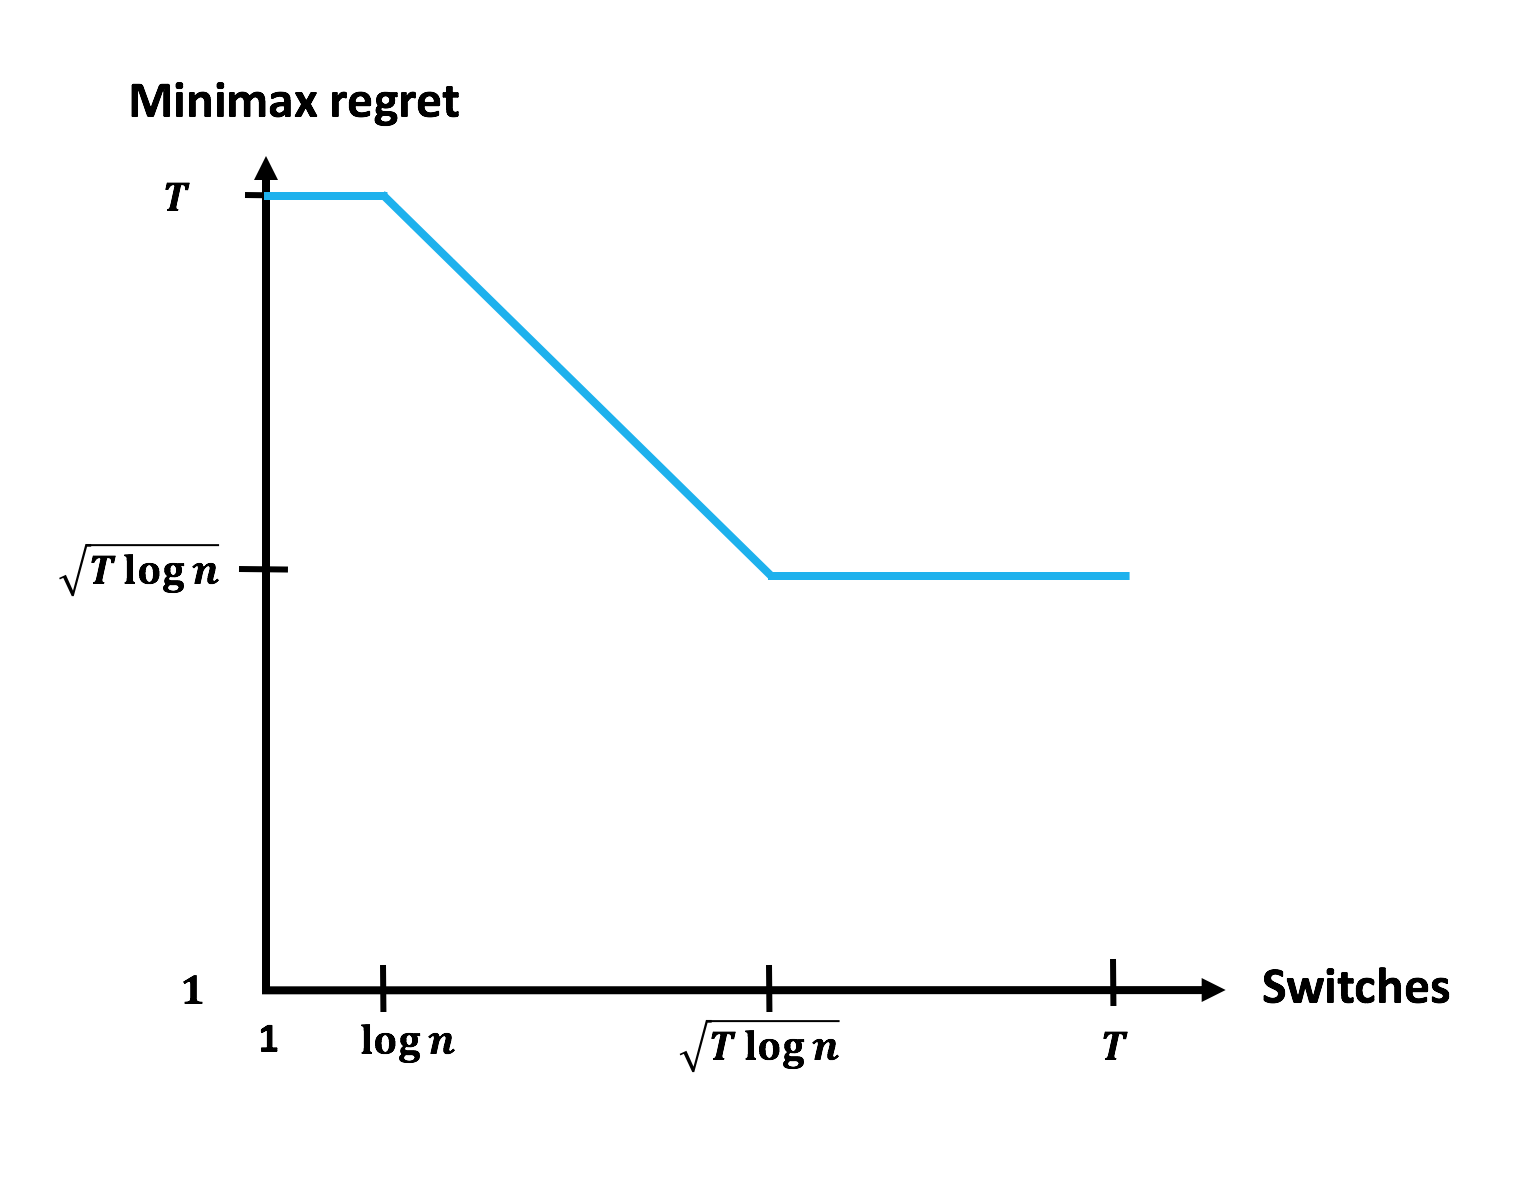
\includegraphics[width=70mm]{figure_pfe.png}}
\subfigure[Switching-budget MAB.]{\label{fig:mab}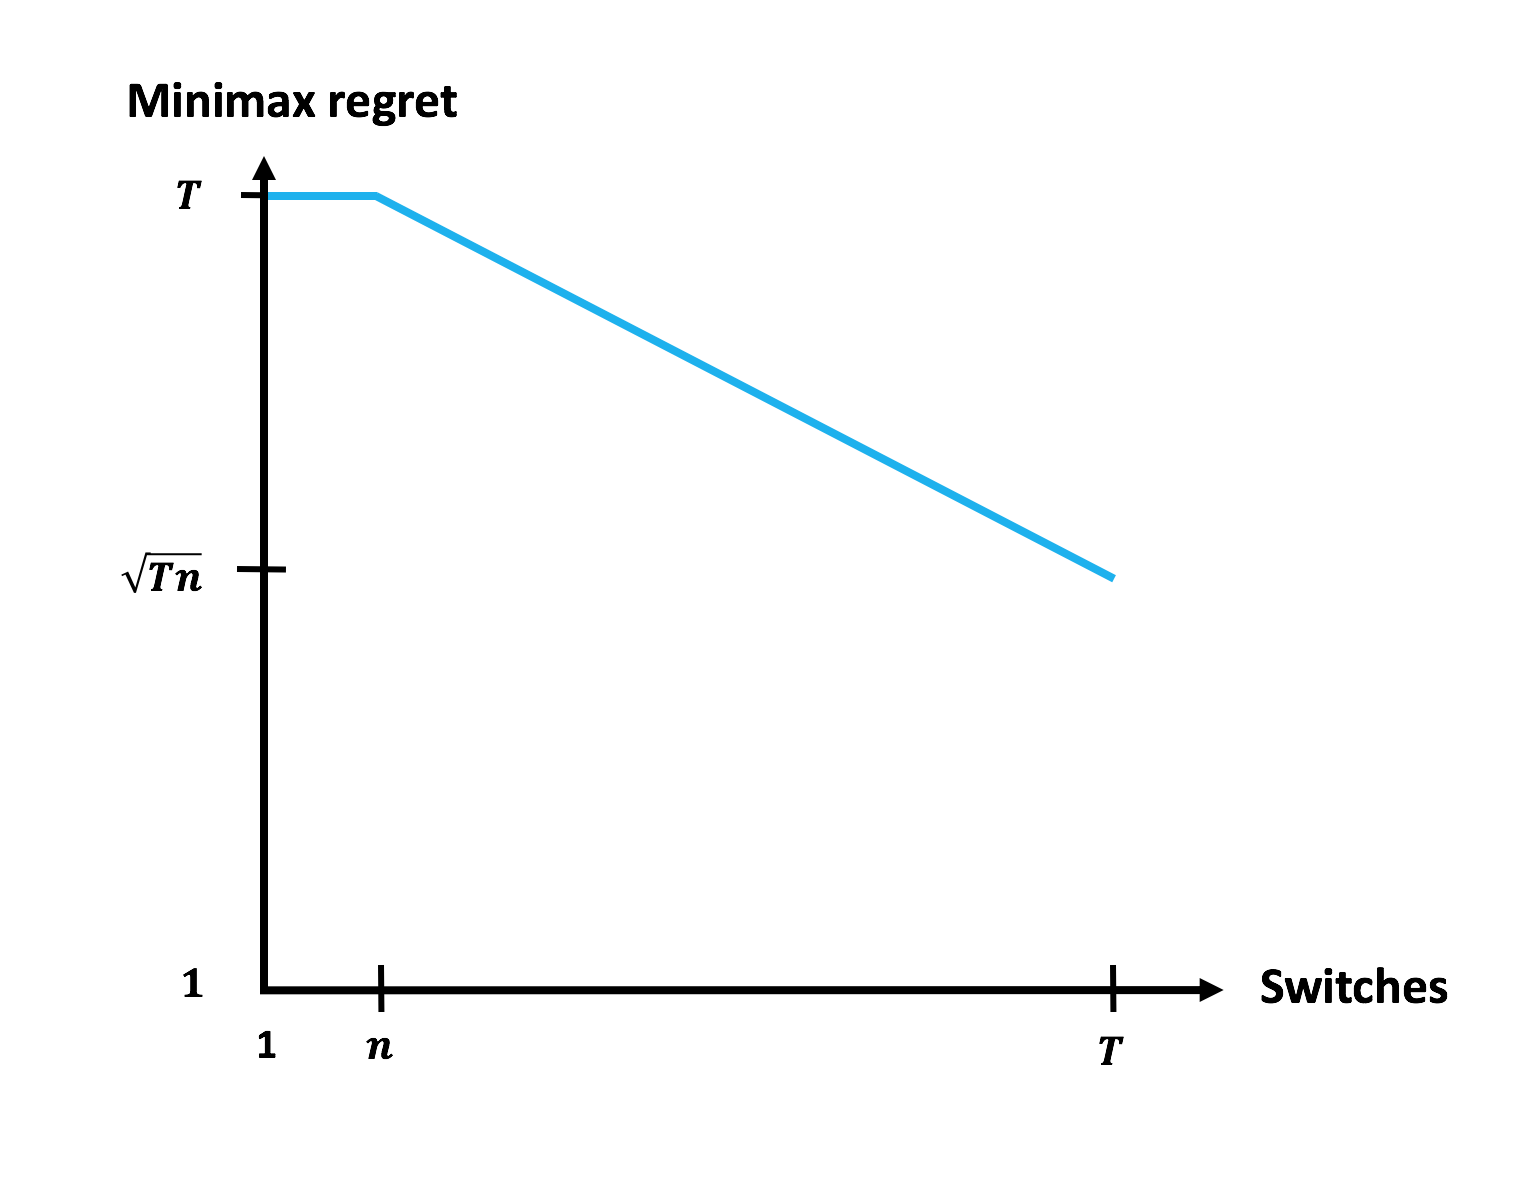
\includegraphics[width=70mm]{figure_mab.png}}
\caption{Complexity landscape of online learning over a finite action set with limited switching. Axes are plotted in log-log scale. Polylogarithmic factors in $T$ are hidden for simplicity.}
\label{fig:plots}
\end{figure}

\subsection{Our contributions}\label{subsec:intro-contributions}
%The goal of this paper is to better understand the value of switching in online learning over a finite action set.

We present the first algorithms for switching-cost PFE that achieve the minimax optimal rate $O(\sqrt{cT\log n})$ with high probability. In fact, our results are more general: we give a framework to formulaically convert algorithms that work in expectation and fall under the Follow-the-Perturbed-Leader algorithmic umbrella, into algorithms that work with high probability. We also show how this framework extends to online combinatorial optimization, i.e. online linear optimization over a combinatorial polytope, where offline optimization can be done efficiently. 

\par We also investigate the \textit{switching budget} setting for the PFE and MAB problems. The above result and standard reductions allow us to completely characterize the complexity of this switching budget setting up to small polylogarithmic factors: for both the PFE and MAB problems, for all switching budgets $S \leq T$, and for both expectation and high probability guarantees. For PFE, we show the optimal rate is of order $\tilde{\Theta}(\sqrt{T\log n})$ for $S = \Omega(\sqrt{T\log n})$, and $\min(\tilde{\Theta}(\tfrac{T\log n}{S}), T)$ for $S = O(\sqrt{T \log n})$. Interestingly, the bandit setting does not exhibit such a phase transition; instead we show the minimax rate decays steadily as $\min(\tilde{\Theta}(\frac{T\sqrt{n}}{\sqrt{S}}), T)$ for all ranges of $S \leq T$.%\footnote{The lower bound is implicitly implied by~\citep{DekDinKorPer}, but without the correct dependency on $n$; see Section~\ref{sec:budgets-mab}.}

.

\section{Acknowledgements.} We are indebted to Elad Hazan for numerous fruitful discussions and for suggesting the switching-budget setting to us. We also thank Yoram Singer, Tomer Koren, David Martins, Vianney Perchet, and Jonathan Weed for helpful discussions.
\par Part of this work was done while JA was visiting the Simons Institute for the Theory of Computing, which was partially supported by the DIMACS/Simons Collaboration on Bridging Continuous and Discrete Optimization through NSF grant \#CCF-1740425. JA is also supported by NSF Graduate Research Fellowship 1122374.


%\newpage
%\addcontentsline{toc}{section}{References}
\bibliography{bibSwitching}



\end{document}
